\documentclass[lettersize,journal]{IEEEtran}
\usepackage{amsmath,amsfonts}
\usepackage{algorithmic}
\usepackage{algorithm}
\usepackage{array}
\usepackage[caption=false,font=normalsize,labelfont=sf,textfont=sf]{subfig}
\usepackage{textcomp}
\usepackage{stfloats}
\usepackage{url}
\usepackage{verbatim}
\usepackage{multirow}
\usepackage{graphicx}
\usepackage{cite}
\hyphenation{op-tical net-works semi-conduc-tor IEEE-Xplore}
% updated with editorial comments 8/9/2021

\begin{document}

\title{Gesture Command: A Camera-Based Gesture Recognition system for British and American Sign Language}

\author{Malayah Powlette, Student number: 2292564}
        % <-this % stops a space

% The paper headers
\markboth{LH/LM Intelligent Robotics final project, No.~1, December~2025}%
{Shell \MakeLowercase{\textit{et al.}}: A Sample Article Using IEEEtran.cls for IEEE Journals}

\maketitle

\begin{abstract}
This paper navigates a robot simulation of a robot in a setting such as a grocery store which would in theory have a map of the store and assist and navigate  specifically mute, death and hard of hearing customers. The paper will discuss the limitations to such a program, thorough testing of said program and the guides to repeat such testing.
The problem this paper will be focused on is the lack of accessabily to help for the named communities. 
\\
Sign language is known by the minority and this limits the experiences these groups have and make the experiences they do that much more difficult. It's unrealistic to believe we as people could or would learn sign language for the minority. This is why I strongly believe that the creation of programs that can understand and translate sign language are extremely important, and it would be incredible to see similar and far more advanced programs implemented in the future. Whether these implementations be in schools, shops or any other useful areas. My program is ran through a \textbf{\textit{Python}} file on \textbf{\textit{Visual Studio Code}} that has the code for the sign recognition and starts a pre-setup simulation in \textbf{\textit{Coppeliasim}}. 
\end{abstract}

\section{Introduction}
\IEEEPARstart{I}{n} this document i will be discussing my project to create a robot program that can understand a pre-inputted list of sign language gestures in both American sign language and British sign language. My aim was for the robot’s program to allow it to input sign language gestures from a human participant and translate what they are saying word by word. My reasoning for choosing the project stems from the fact that, during the covid lock downs, I took a strong interest in sign language and grew a great passion to be able to communicate in it. Sadly I did not keep steady in my learning and have been unsuccessfully aiming since to re-learn. I believe learning sign language is so important in our communities for inclusion and that it is simply an amazing and useful skill to have under your belt. Due to this, I have taken this project as my opportunity to push myself to re-learn the language and implement my learnings into a program that will understand and translate inputted information from both British and American sign language.  

\section{Related work}
From the research I have conducted, I have found numerous shopping assistant robots simply for assistance of the average customer. One example i have found is the \textbf{\textit{Spod}} robot. This robot is aimed to be placed in shops to help customers navigate the store to desired products. There however do not appear to be any shopping assistants that catter to the deaf and hard of hearing communities. It's not lost on me that these are only the first implimentations of these robots and it would be assumed and hoped that these accessibility feactures would be implemented in their  future roll out. As for this project, i chose to use my own resources and did not look towards these existing robots for inspiration.

\section{The Software used }

From my research into robot simulations, I found that \textbf{\textit{Coppeliasim}} was a well suggested simulation for this kind of project. The application comes with the tools to use pre-existing robots or to generate your own. As it was not expected of me to make my own robot for this project, I chose from those provided. The application has a vast library of objects for simulations and I was able to pick through these to create the desired environment for my simulation and robot needs. As i have never worked with robots before, I used numerous youtube videos and online websites as tutorials to navigate my way through the program. The bulkier portion of my code was the implementation of  a sign language recognition program and i decided to code this in \textbf{\textit{Python}} as I am well versed in the language and many similar projects seemed to use this language. 
\section{Method }

To implement my project, I first focused on the Sign Language recognition in Python, as I knew this would need the most time to be rendered. 
\\
\\
Collect\_imgs.py coding:
\begin{enumerate}
\item{ I first took to accessing the laptop camera and using  \textbf{\textit{cv2}} to create a frame and constantly present the current image from the camera to give the impression of a video. I implemented code that would, for each sign in the np array "signs", allow the user to enter "S" once they are ready to demonstrate said sign and for each sign would take 30 sets of 30 images and each set of 30 images would in esence be a video of the current sign. The code would then write all of the extracted landmark positions to the "data" folder, each subsequently split up by sign, squence number and finally by image   }
\item{Next, I used matplot to train my sign recognition program. I did this by accessing and using all of the position point locations from the "data" file and linking each "video" to its sign. }
\item{I then stored this training data to the "model.p" file to be accessed in the main code later}


\end{enumerate}

Control\_robot2.py sign recognition coding: 
\begin{enumerate}
\item{To then create the code to translate the sign language, I then implemented the same code for entering in the signs and marking the landmark positions. I coded the program to then take thirty images from the screen once "S" was entered.  }
\item{In the start of my code i open the model file and save it as a models dictionary. After the 30 images have been rendered, I use the model's predict function for the program to give the guess of what sign has been entered by the user }

\end{enumerate}

Robot.ttt Creating the simulation: 
\begin{enumerate}
\item{ To start creating my simulation, I had to decide on my robot. I chose from the mobile robots as it was a key factor that my robot had to move. After playing with a couple of the options, I chose to use NAO as it seemed the easiest to program to follow a path.   }
\item{ After this, I got started on loooking through the objects I could add for the robot to have to navaigate to and ended up adding a bowl and a cup to the scene. I then created two paths, one to each item; both starting at the robots location.}
\item{I then deactivated the JointRecorder script in NAO that had control of its current movements }
\item{Next, after researching how to make an object follow a path in Coppeliasim, I made two functions in the NAO script. The functions are the same with the only difference being which path the robot will follow. The functions make the robot take a "step" along the desired path when called.  }
\end{enumerate}

Control\_robot2 Implementing the Remote API: 
\\
Finally, I had to link the sign language recognition to the simulation 
\begin{enumerate}
\item{ I first used the coppeliasim ZMQ remote api to make a connection to the simulation}
\item{Following this,  I programed the sign reader to return either a 0 for bowl or a 1 for cup. Based on the item signed for, the {\it{ callScriptFunction}} Function would call the function to follow the intended path from the script which I called using the {\it{ getObject} }Function }

\end{enumerate}


\section{Algorithms}


Link to the software repository:


\begin{algorithm}[H]
\caption{Sign recognition code.}\label{alg:alg1}
\begin{algorithmic}
\STATE 
\STATE \hspace{0.5cm}$ \textbf{while cap.isOpened(): }  $
\STATE \hspace{0.5cm}$ \textbf{\quad ret, frame = cap.read() }  $
\STATE \hspace{0.5cm}$ \textbf{\quad image, results = mediapipe\_det(frame, holistic) }  $
\STATE \hspace{0.5cm}$ \textbf{\quad cv2.putText(frame, 'Ready? Press "S" ! :)', (100, 50), }  $
\STATE \hspace{0.5cm}$ \textbf{\quad \quad cv2.FONT\_HERSHEY\_SIMPLEX, 1.3, (0, 255, 0), 3, cv2.LINE\_AA) }  $

\STATE \hspace{0.5cm}$ \textbf{\quad cv2.imshow('Sign render frame', frame) }  $
\STATE \hspace{0.5cm}$ \textbf{\quad if cv2.waitKey(10) == ord('s'): }  $

\STATE \hspace{0.5cm}$ \textbf{\quad \quad counter = 0 }  $
\STATE \hspace{0.5cm}$ \textbf{\quad \quad s=[] }  $
\STATE \hspace{0.5cm}$ \textbf{\quad \quad while counter < 30: }  $
\STATE \hspace{0.5cm}$ \textbf{\quad \quad \quad ret, frame = cap.read() }  $
\STATE \hspace{0.5cm}$ \textbf{\quad \quad \quad cv2.imshow('Sign render frame', frame) }  $
\STATE \hspace{0.5cm}$ \textbf{\quad \quad \quad s.append(extractLMs(results)) }  $
\STATE \hspace{0.5cm}$ \textbf{\quad \quad  \quad cv2.waitKey(20) }  $
\STATE \hspace{0.5cm}$ \textbf{\quad \quad \quad counter += 1 }  $

\STATE \hspace{0.5cm}$ \textbf{\quad \quad for i in range (30): }  $
\STATE \hspace{0.5cm}$ \textbf{\quad \quad  \quad sign.append((np.array(s))) }  $

\STATE \hspace{0.5cm}$ \textbf{\quad \quad nsamples, nx, ny = np.array(sign).shape }  $
\STATE \hspace{0.5cm}$ \textbf{\quad \quad d2\_sign = np.array(sign).reshape((nsamples,nx*ny))   }  $
\STATE \hspace{0.5cm}$ \textbf{\quad \quad result = mode( model.predict((np.array(d2\_sign)))) }  $
\STATE \hspace{0.5cm}$ \textbf{\quad \quad break }  $


\end{algorithmic}
\label{alg1}
\end{algorithm}

\begin{algorithm}[H]
\caption{Robot path follolwing code.}\label{alg:alg2}
\begin{algorithmic}
\STATE 
\STATE \hspace{0.5cm}$ \textbf{function bowl\_path() }  $

\STATE \hspace{0.5cm}$ \textbf{\quad sim = require('sim') }  $
\STATE \hspace{0.5cm}$ \textbf{\quad objectToFollowPath = sim.getObject('..') }  $
\STATE \hspace{0.5cm}$ \textbf{\quad path = sim.getObject('/Path[0]') }  $
\STATE \hspace{0.5cm}$ \textbf{\quad pathData = sim.unpackDoubleTable(sim.getBufferProperty(path, 'customData.PATH')) }  $
\STATE \hspace{0.5cm}$ \textbf{\quad local m = Matrix(\#pathData // 7, 7, pathData) }  $
\STATE \hspace{0.5cm}$ \textbf{\quad pathPositions = m:slice(1, 1, m:rows(), 3):data() }  $
\STATE \hspace{0.5cm}$ \textbf{\quad pathQuaternions = m:slice(1, 4, m:rows(), 7):data() }  $
\STATE \hspace{0.5cm}$ \textbf{\quad pathLengths, totalLength = sim.getPathLengths(pathPositions, 3) }  $
\STATE \hspace{0.5cm}$ \textbf{\quad     velocity = 0.04 -- m/s) }  $
\STATE \hspace{0.5cm}$ \textbf{\quad posAlongPath = 0}  $
\STATE \hspace{0.5cm}$ \textbf{\quad previousSimulationTime = 0}  $
\STATE \hspace{0.5cm}$ \textbf{\quad sim.setStepping(true) }  $

\STATE \hspace{0.5cm}$ \textbf{\quad \quad local t = sim.getSimulationTime() }  $
\STATE \hspace{0.5cm}$ \textbf{\quad \quad posAlongPath = posAlongPath + velocity * (t - previousSimulationTime) }  $
\STATE \hspace{0.5cm}$ \textbf{\quad \quad posAlongPath = posAlongPath \% totallength}  $
\STATE \hspace{0.5cm}$ \textbf{\quad \quad local pos = sim.getPathInterpolatedConfig(pathPositions, pathLengths, posAlongPath) }  $
\STATE \hspace{0.5cm}$ \textbf{\quad \quad  local quat = sim.getPathInterpolatedConfig(pathQuaternions, pathLengths, }  $
\STATE \hspace{0.5cm}$ \textbf{\quad \quad \quad posAlongPath, nil, \{2, 2, 2, 2\}) }  $
\STATE \hspace{0.5cm}$ \textbf{\quad \quad sim.setObjectPosition(objectToFollowPath, pos, path) }  $
\STATE \hspace{0.5cm}$ \textbf{\quad \quad sim.setObjectQuaternion(objectToFollowPath, quat, path) }  $
\STATE \hspace{0.5cm}$ \textbf{\quad \quad previousSimulationTime = t}  $
\STATE \hspace{0.5cm}$ \textbf{\quad \quad sim.step() }  $

\STATE \hspace{0.5cm}$ \textbf{end }  $

        

\end{algorithmic}
\label{alg2}
\end{algorithm}

\section{Testing the project}

\subsection {Running the code}

\begin{list}{}{}
\item{Open \texttt{robot.ttt}}
\item{Open  \texttt{control\_robot}}
\item{Run \texttt{control\_robot2}}
\end{list}



\subsection {Signs for code testing}
Fig. 1demonstrate the sign langauge for bowl. The sign is the same in both British and American sign language .

Fig. 2 and Fig. 3 demonstrate the sign langauge for cup in both British sign language and American sign language respectively.

\begin{figure}[h]
\centering
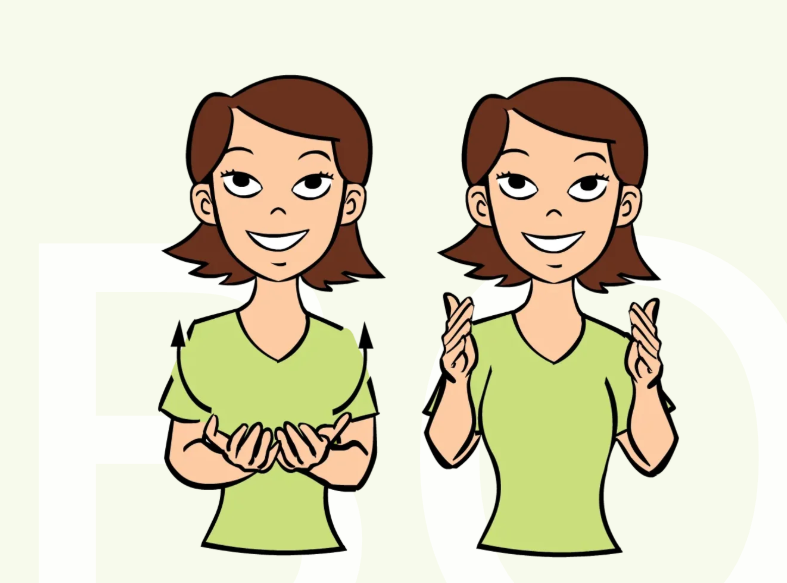
\includegraphics[width=2.5in]{pic1}
\caption{Sign for Bowl.}
\label{fig_1}
\end{figure}

\begin{figure}[h]
\centering
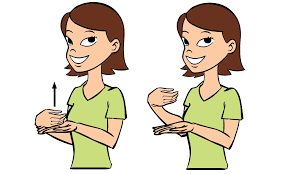
\includegraphics[width=2.5in]{pic2}
\caption{Sign for cup ASL.}
\label{fig_2}
\end{figure}

\begin{figure}[h]
\centering
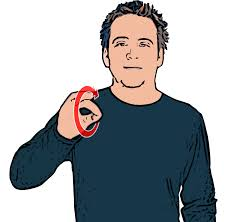
\includegraphics[width=2.5in]{pic3}
\caption{Sign for cup BSL.}
\label{fig_3}
\end{figure}


\subsection{Experimental results }

To test my code I repetadly ran the program and signed either for a cup or bowl. I then recorded the sign detections interpretation of my sign and recorded these results in a table.I repeated this test 20 times. During the test, i commented out the calling to the robot simulator as that was not the focus of this test. The results are in the table below. I then calculated the accuracy of these tests and it resulted in an accuracy of  \texttt{??\%}
\hfill \break

\begin{tabular}{ |p{2cm}|p{2cm}|p{2cm}|}
 \hline
 \multicolumn{3}{|c|}{Sign Test} \\
 \hline
 TEST NO&SIGN &RESULT\\
 \hline
 Afghanistan   & AF    &AFG\\
 Aland Islands&   AX  & ALA  \\
 Albania &AL & ALB\\
 Algeria    &DZ & DZA\\
 American Samoa&   AS  & AS\\
 Andorra& AD  & AND   \\
 Angola& AO  & AG\\
 \hline
\end{tabular}
\\
To test my robot was correctly following the path, I uncommented the code to connect to the simulation and ran the program repeatedly once again.  I would ignore weither the program accurately recognise my sign and this time record the sign that the program had recognised.  Then i would view the simulation and assure that this was the object that the robot would travel to. The robot followed the correct path each time.
\hfill \break



\section{Conclusion}

In Conclusion, through this project I was able to create a functioning robot simulation that could take in sign langauge and guide a user to an object within it's vocabulary. My testing demonstrates that this program is quite accurate and I believe in the future this will be a real robot and implemented in situations all around us. I would have loved to have a much broader library to fully put this robot to the test. If i were to do this project again I would definetly find a different robot simulator as there was not much information and assistance online for Coppeliasim. If I were to do this project in my own time, I would also have the luxury of not being under  a time crunch and would be able to perfect the simulation and create the best and most applicable to the real world simulation i could. As the simulation works well and seems it would be a useful and inteligent tool in the real world I am however happy with the result and proud of what i have produced.

\subsection{Limitations}

During my project I was met with multiple limitations along the way. Despite the limitations, I could still produce a functional simulation with my intended results. The limitations I came across are as follows:

\begin{list}{}{}
\item{The lack of shopping products in CoppeliaSim: This limitation does not affect the actual project, however it did limit my ability to show the distinctions being made by the sign recognition. Although, given the clear difference in the signs for bowl and cup, this is still clearly portrayed.}
	
\item{My lack of knowledge in robot simulations and difficulty finding information on specific tools: This limitation meant that tasks like making the robot follow paths and calling functions using an API took me much longer than an experienced coder would have and this having consumed my time meant that I had none spare to make the simulation as good as it could've been and resulted in the robot not being programmed specifically to use all of it's joints whilst following the path. }
\item{Failure to access robot camera and a  lack of body model to use if I had access to the camera: In my origional plan for this project, I aimed to use the simulated robot's vision sensors to retrieve the sign language. I was unsuccessful in finding how to access this camera though and subsequently stuck to the computer's camera. This did however have me stuck attempting to do this for a while. I later realised that had I been able to access the camera, There were no objects that I would have been able to use for the sign language anyways. All in all this was simply  a big loss of time at no success.  }
\item{API implimentation means that when functions are called externally, the simulation is paused until the function is completed: This resulted in me having to put the while count loop in the python file. Realistically this would remain in the robot's functions, but for a better representation, I have decided to implement it in this way.   }


\end{list}


\section*{Acknowledgments}

\begin{list}{}{}
\item{{\it{moving Sign recognition tutorial}}. https://youtu.be/doDUihpj6ro?si=wEawHBzHJXBlnwo8}
\item{{\it{ Sign recognition tutorial}}. https://www.youtube.com/watch?v=MJCSjXepaAM}
\item{\it{ Path following code }. https://manual.coppeliarobotics.com/en/paths.htm}
\end{list}


\section{References Section}

\begin{thebibliography}{1}
\bibliographystyle{IEEEtran}

\bibitem{ref1}
{\it{Bowl sign}}. https://babysignlanguage.com/dictionary/bowl/

\bibitem{ref2}
{\it{ Cup sign asl}}. https://babysignlanguage.com/dictionary/cup/

\bibitem{ref3}
{\it{Cup sign bsl}}. https://www.british-sign.co.uk/british-sign-language/how-to-sign/tea/
\bibitem{ref4}
{\it{Spod robot}}. https://www.youtube.com/watch?v=7zfjawHkD00

\end{thebibliography}


\newpage


\end{document}


